\documentclass[a4paper,11pt]{article}
\usepackage{latexsym}
\usepackage[utf8]{inputenc}
\usepackage[activeacute,spanish]{babel}
\usepackage{lineno}
\usepackage{amsmath}
\RequirePackage{graphicx}
\RequirePackage{booktabs}
\RequirePackage{textpos}
\usepackage{graphicx}
\graphicspath{{figuras/}} % Carpeta de imágenes

\usepackage[colorlinks,linkcolor={blue},citecolor={blue}]{hyperref}
\hypersetup{urlcolor=blue, colorlinks=true} % Colors hyperlinks in blue

\linespread{1.2} % Interlineado
%\setlength{\parindent}{0pt} % Elimina la sangría
\usepackage{geometry} % Control de margenes
\geometry{left=1.5cm, right=2.0cm, top=2.2cm, bottom=2.2cm}

%opening
\title{Teorema de Noether}
\author{Jhemerson Alvarado \\
 Universidad Nacional Mayor de San Marcos, Lima Perú \\
\emph{jhemerson.alvarado@unmsm.edu.pe}\\}
\date{}

\begin{document}


%\linenumbers % Coloca numeracion a las lineas
\maketitle
%\logo{Orcid}
 \begin{textblock*}{297mm}(56.0mm,-28.4mm)
	\href{https://orcid.org/0009-0004-8141-3241}{
	
\includegraphics[scale=0.033]{orcid}}
\end{textblock*}


\begin{abstract} \noindent 
%redactar el resumen:
Se abordó la derivación del teorema de Noether a través del Principio de Acción Estacionaria. Esta derivación siguió una estructura similar a la presentada en la teoría de campos clásica, enfatizando la importancia de las propiedades de invariancia de la acción. Se destacó que las transformaciones de simetría asociadas operan en trayectorias, no en puntos del espacio y el tiempo. El trabajo también incluyó una exposición de la biografía de Noether.



\textbf{Palabras clave}: Principio de Acción Mínima, Leyes de conservación, Lagrangiano, Invariancia
\end{abstract}

 
\renewcommand{\abstractname}{Abstract}


\begin{abstract} \noindent		
%traducir:
The derivation of Noether's theorem was addressed through the Principle of Stationary Action. This derivation followed a structure similar to that presented in classical field theory, emphasizing the importance of the invariance properties of the action. It was highlighted that the associated symmetry transformations operate on trajectories, not on points in space and time. The work also included an exposition of Noether's biography.\\
\textbf{Keywords}: Least action principle, Conservation Laws, lagrangian, Invariance
\end{abstract}



%%%%%%%%%%%%%%%%%%%%%%%%

\section{Introducción}
Ser el epónimo de un adjetivo es el más alto reconocimiento que puede recibir un matemático, incluso más significativo que la concesión de la Medalla Fields. Mientras la geometría euclidiana evoca a Euclides, las coordenadas cartesianas llevan el nombre de Descartes, y la mecánica newtoniana rinde homenaje a Newton, Emmy Noether ha dejado su propio legado lingüístico con los anillos noetherianos. Hasta donde tengo conocimiento, Emmy Noether es la única mujer matemática que ha alcanzado este honor, siendo indiscutiblemente la primera en lograrlo.\cite{Volker}
\\
En 1918, Albert Einstein comunicó a David Hilbert su impresión positiva sobre el trabajo de Emmy Noether en la generación de invariantes: \textit{“Ayer recibí de la señorita Noether un trabajo muy interesante sobre la generación de invariantes. Estoy impresionado de que estos asuntos se puedan entender desde un punto de vista tan general. La vieja guardia de Göttingen debería aprender de la señorita Noether. Verdaderamente sabe lo que hace”}\cite{Valenzuela}. De esta manera, Einstein describió a la científica Emmy Noether, quien enfrentó obstáculos significativos, incluidos desafíos políticos durante la ascensión del régimen nazi en Alemania.
\\

La relación entre simetría y leyes de conservación es fundamental. El teorema de Noether desempeña un papel central en la teoría de campos clásica al abordar este tema de manera unificada. El concepto de acción se utiliza para presentar el teorema, conectándolo con las propiedades de invariancia de la acción. El concepto de acción se adapta bien a este propósito y, de hecho, varios libros de texto\cite{Goldstein} y artículos.\cite{Hill} 
Se detalla una presentación más unificada del teorema de Noether, destacando la importancia de las transformaciones del tiempo y las coordenadas en este marco.





%%%%%%%%%%%%%%%%%%%%%%%
%\section{Datos}
\section{Historia y Antecedentes}
\subsection{Vida de Amalie Emmy Noether}


\begin{itemize}
		\item Amalie Emmy Noether, la mayor de tres hermanos e hija del matemático Max Noether, nació el 23 de marzo de 1882 en Erlangen, Baviera, en el seno de una familia judía acomodada con una sólida tradición matemática. Desde una edad temprana, desarrolló una pasión por las matemáticas al vivir en un entorno impregnado de esta disciplina, influenciada no solo por sus padres, sino también por los colegas de su padre.
%%%%%%%%%%%%%%%%%%%%%%%%%%%%%%%%%%%%%%%%%%%%%%%%%%%%%%%%%%%%%%%%%%%
        \begin{figure}[h]
         \centering{\includegraphics[scale=0.21]{Emmy_Noether.eps}}
              \caption{\textit{Emmy Noether (1882 - 1932)}}
          \label{figura2}
        \end{figure}  
        \item Sus primeros pasos en la universidad fueron como oyente en la Universidad de Erlangen, que inicialmente no aceptaba mujeres. Sin embargo, Emmy Noether superó el examen de acceso el 14 de julio de 1903. En 1904, la Universidad de Erlangen aceptó su ingreso, convirtiéndose así en la primera mujer en acceder a la institución. Tres años después, en 1907, defendió su tesis, ganando el reconocimiento y estima de su maestro, Paul Gordan, aquel apodado ``El rey de los invariantes"

        \item A pesar de los intentos de los matemáticos David Hilbert y Felix Klein por lograr la habilitación de Noether en la Universidad de Göttingen, enfrentaron numerosas críticas. En una de ellas, Hilbert respondió diciendo:``Señores míos, no encuentro que el género de la candidata sea un motivo válido en contra de su aceptación como profesora. Después de todo, la junta no es una casa de baños" \cite{Valenzuela}. Aunque el claustro dio su voto a favor de su ingreso, la administración no lo permitió. Sin embargo, se aceptó que Noether dictara las clases sobre "Teoría de Invariantes" de Hilbert, durante el período de 1916 a 1917 sin tener algún pago monetario. A pesar de los obstáculos, Emmy Noether dejó una huella significativa en la historia de las matemáticas.


        \item Klein y Einstein, así como entre Klein y Hilbert, mantuvieron una frecuente correspondencia en 1917 sobre el problema de la conservación de la energía. Durante estas discusiones, Klein abordó el tema con Emmy Noether, del cual llegaron a la conclusión de que la ley de conservación de la energía no se derivaba directamente de las ecuaciones que describían la gravitación. Noether en 1908 presentó su artículo "Invariante Variationsprobleme”, que describían dos teoremas.

        \item En 1922, la Universidad de Göttingen le otorgó a Emmy Noether el título de profesora extraordinaria,\cite{Freire} lo que le concedió el derecho de llamarse profesora, aunque no estaba acompañado de un salario. Hasta el año 1921, su padre, Max Noether, la sustentaba económicamente, pero al fallecer, Emmy experimentó dificultades financieras. Fue en 1923 cuando la universidad finalmente le asignó una tarea docente remunerada, proporcionándole, por primera vez a los 41 años, un ingreso independiente. Este acontecimiento marcó un hito en la vida de Emmy Noether, reconocida como una destacada investigadora matemática en Alemania y posiblemente a nivel mundial. Los diez años subsiguientes fueron un período de triunfo académico y profesional para ella. En paralelo, se dio una revolución en el ámbito matemático, marcada por un cambio de énfasis desde cálculos y construcciones explícitas hacia enfoques más abstractos y conceptuales. \cite{Volker}

        \item En 1932, Emmy Noether logró una destacada presentación en el Congreso Internacional de Matemáticos en Zúrich, siendo la primera mujer en hacerlo.\cite{Volker}  Sin empleo en ese momento, su situación cambió drásticamente en 1933 cuando, debido a sus opiniones políticas de izquierda y su origen judío, fue despedida en medio de la ascensión del régimen nazi. Optó por un puesto visitante en Bryn Mawr College en Pensilvania, dejando Alemania. 

        \item En 1935, Noether fue intervenida en una cirugía para extirpar un tumor uterino, del cual transcurrió sin problemas, a pocos días empeoró drásticamente y falleció el 14 de abril a la edad de 53 años. En la revista alemana, durante la dominación nazi, Van de Waeren siendo editor, tuvo la valentía de expresar en la revista \textit{"Nuestra ciencia ha sufrido una pérdida trágica"}.\cite{Valenzuela} 

        
\end{itemize}



\subsection{Los Teoremas de Noether}
 
  El primer teorema abordado, se trata de la invarianza de la acción con respecto a las transformaciones del grupo de Lie. La formulación general realizada establece una correspondencia crucial entre las simetrías de un problema variacional y las leyes de conservación que se derivan de las ecuaciones de Euler-Lagrange.
\\
%%%%%%%%%%%%%%%%%%%%%%%%%%%%%%%%%%%%%%%%%%%%%%%%%%%%%%%
        \begin{figure}[h]
         \centering{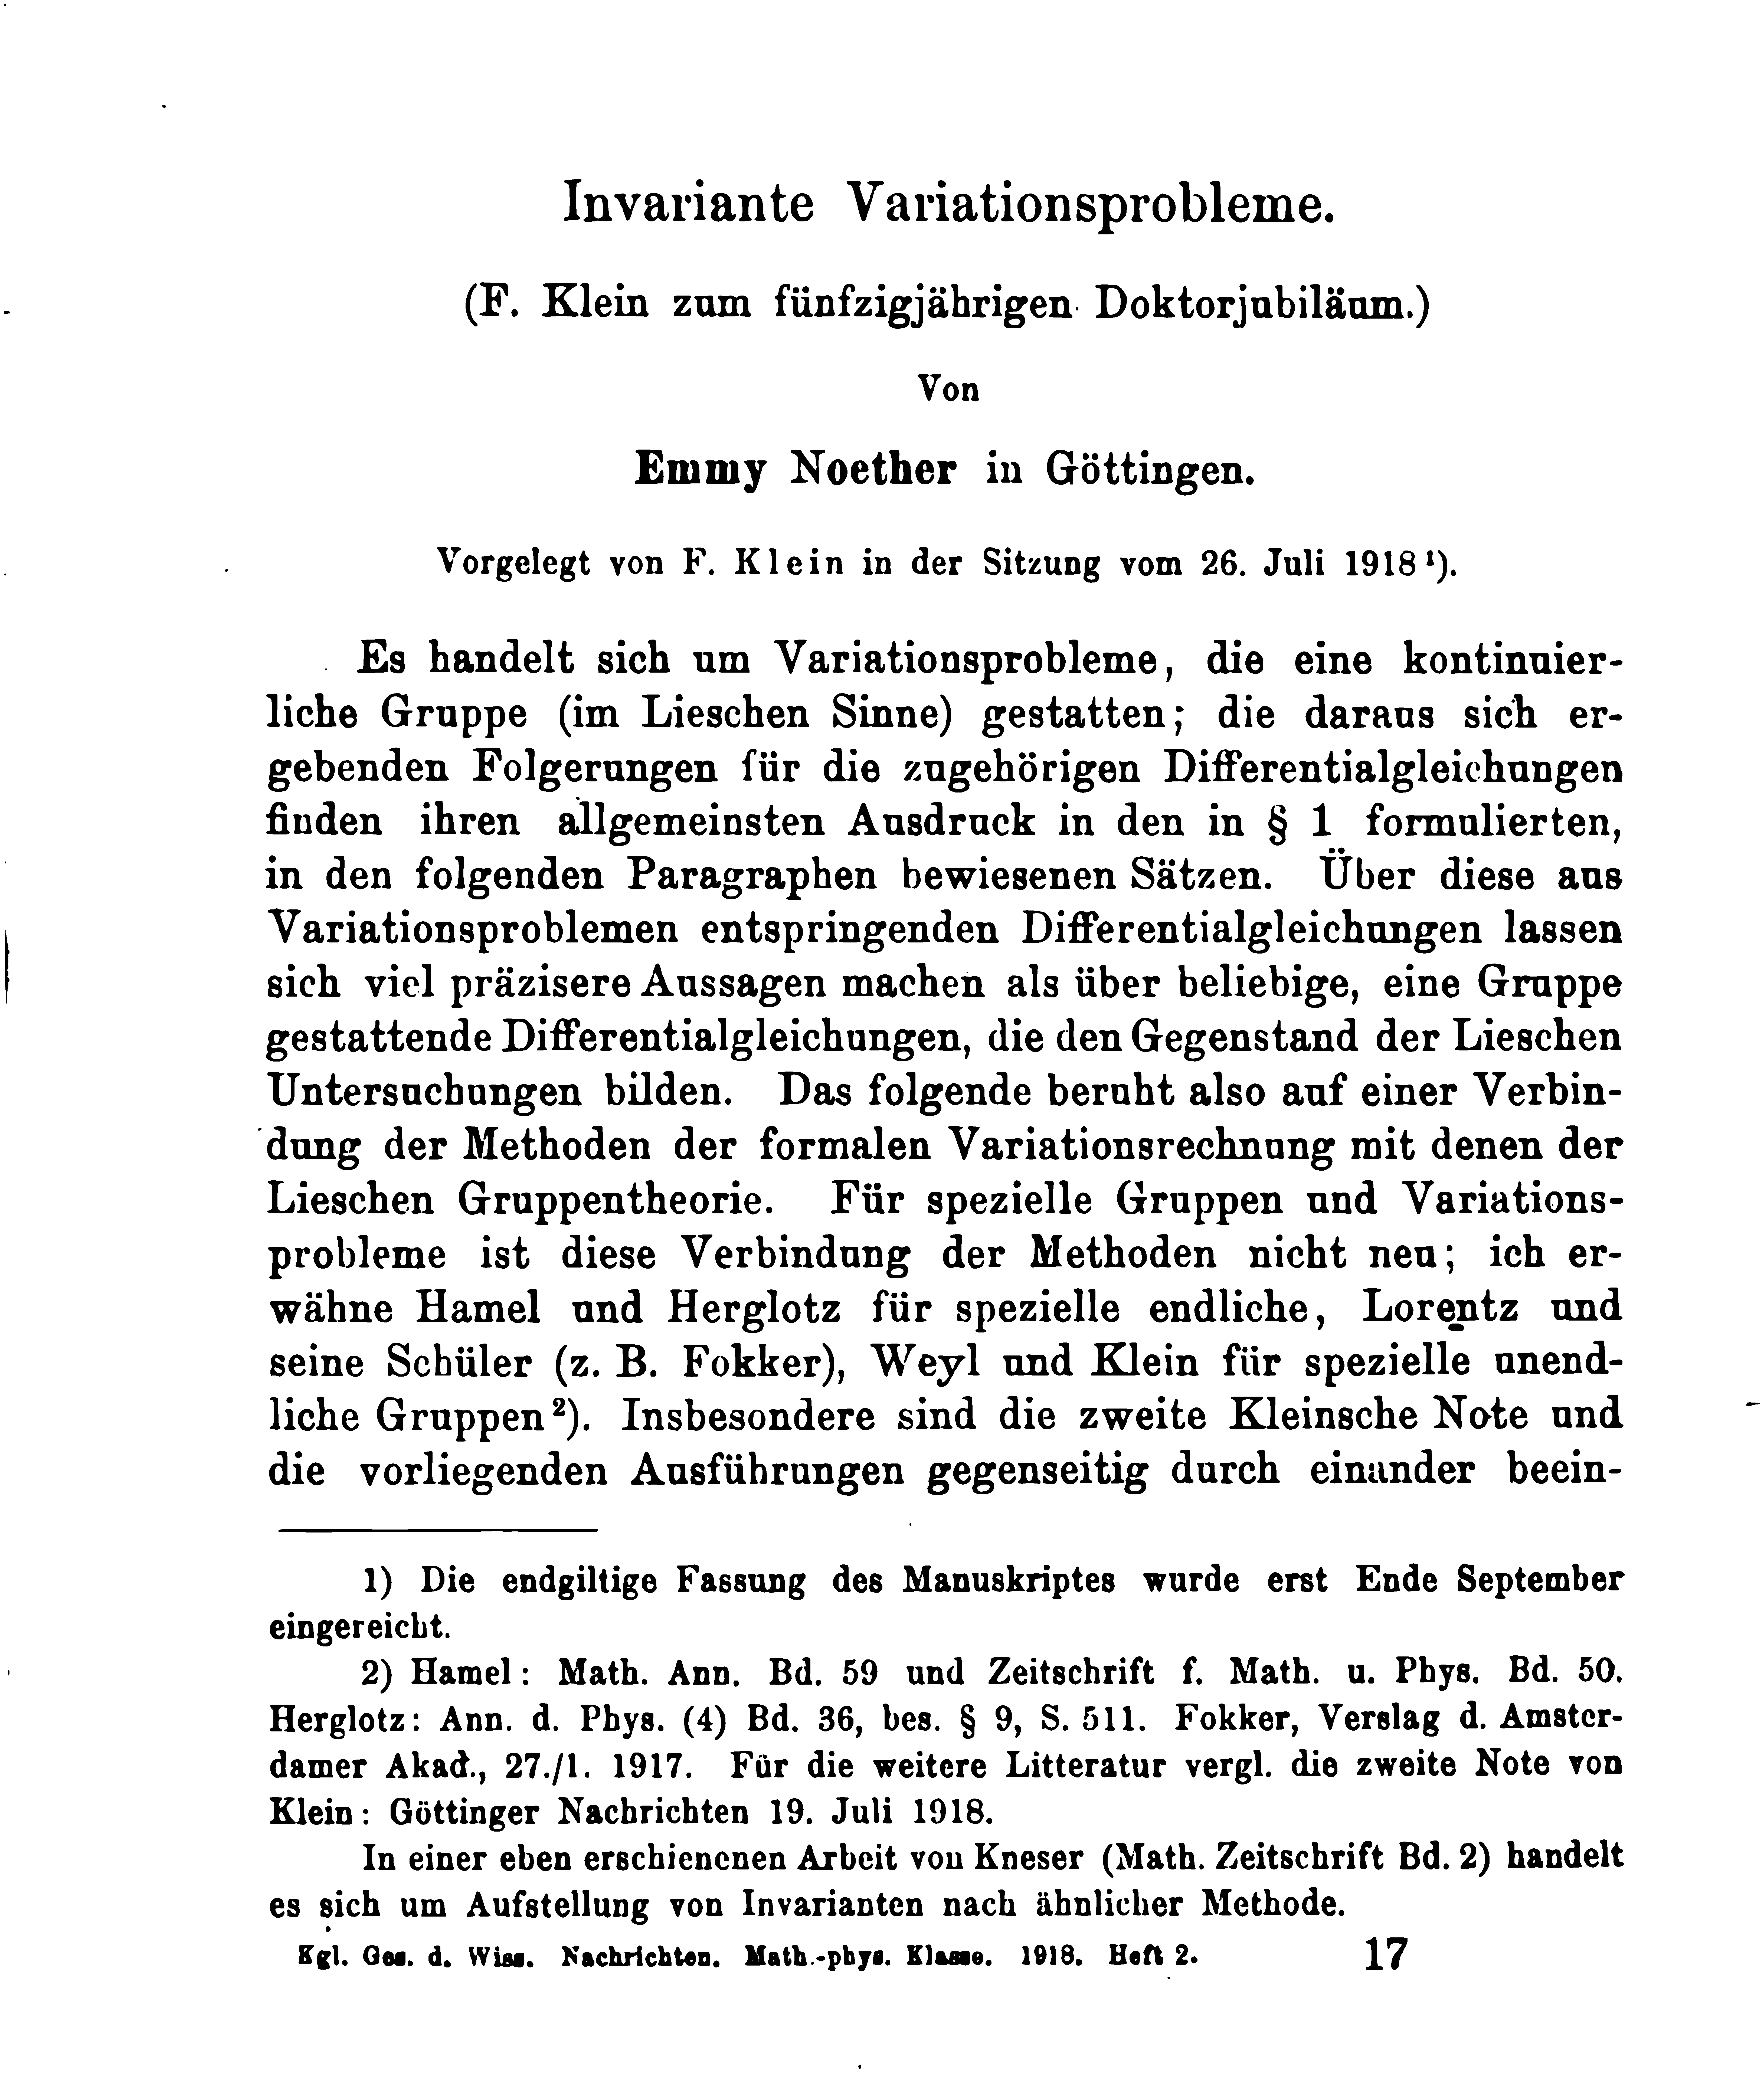
\includegraphics[scale=0.067]{Articulo_de_Noether.eps}}
              \caption{\textit{Artículo de Noether publicado en 1918 ``Invariante Variationsprobleme"}}
          \label{figura2}
        \end{figure}
        
La destacada figura que desarrolló esta teoría proporciona una herramienta invaluable para deducir leyes de conservación si se conocen las simetrías, o para inferir simetrías si se conocen las leyes de conservación. De manera más profunda, el teorema de Noether ofrece un mecanismo para la construcción de la acción, partiendo del conocimiento de las simetrías. En este contexto, se revela que si la acción es invariante frente a un desplazamiento temporal, la energía se conserva. De manera análoga, si la acción es invariante ante un desplazamiento espacial, se conserva el momento lineal. Además, si la invarianza se presenta frente a una rotación, el momento angular se conserva. Finalmente, si la acción es invariante ante una transformación gauge interna, se conserva la carga, y viceversa. Esta interconexión entre simetrías y leyes de conservación ofrece un marco conceptual preciso y poderoso en el ámbito de la física teórica.
\\

En su segundo teorema, Noether aborda la invariancia del problema variacional frente a la acción de un grupo del mismo tipo que se encuentra presente en la teoría de la relatividad general. Esta última es una teoría covariante general, cuyas ecuaciones de campo permanecen invariantes ante cualquier cambio de coordenadas.

En términos más claros, Noether destaca que el problema se comprende de manera más amplia y transparente al utilizar la maquinaria de la teoría de grupos. Además, señala que lo que distingue a la relatividad general es la invariancia del grupo con respecto a funciones arbitrarias que pueden tener dimensiones infinitas, en contraste con el grupo de Lie, que tiene dimensiones finitas.










%imagen del articulo de Noether
%\begin{figure}
%	\centerline{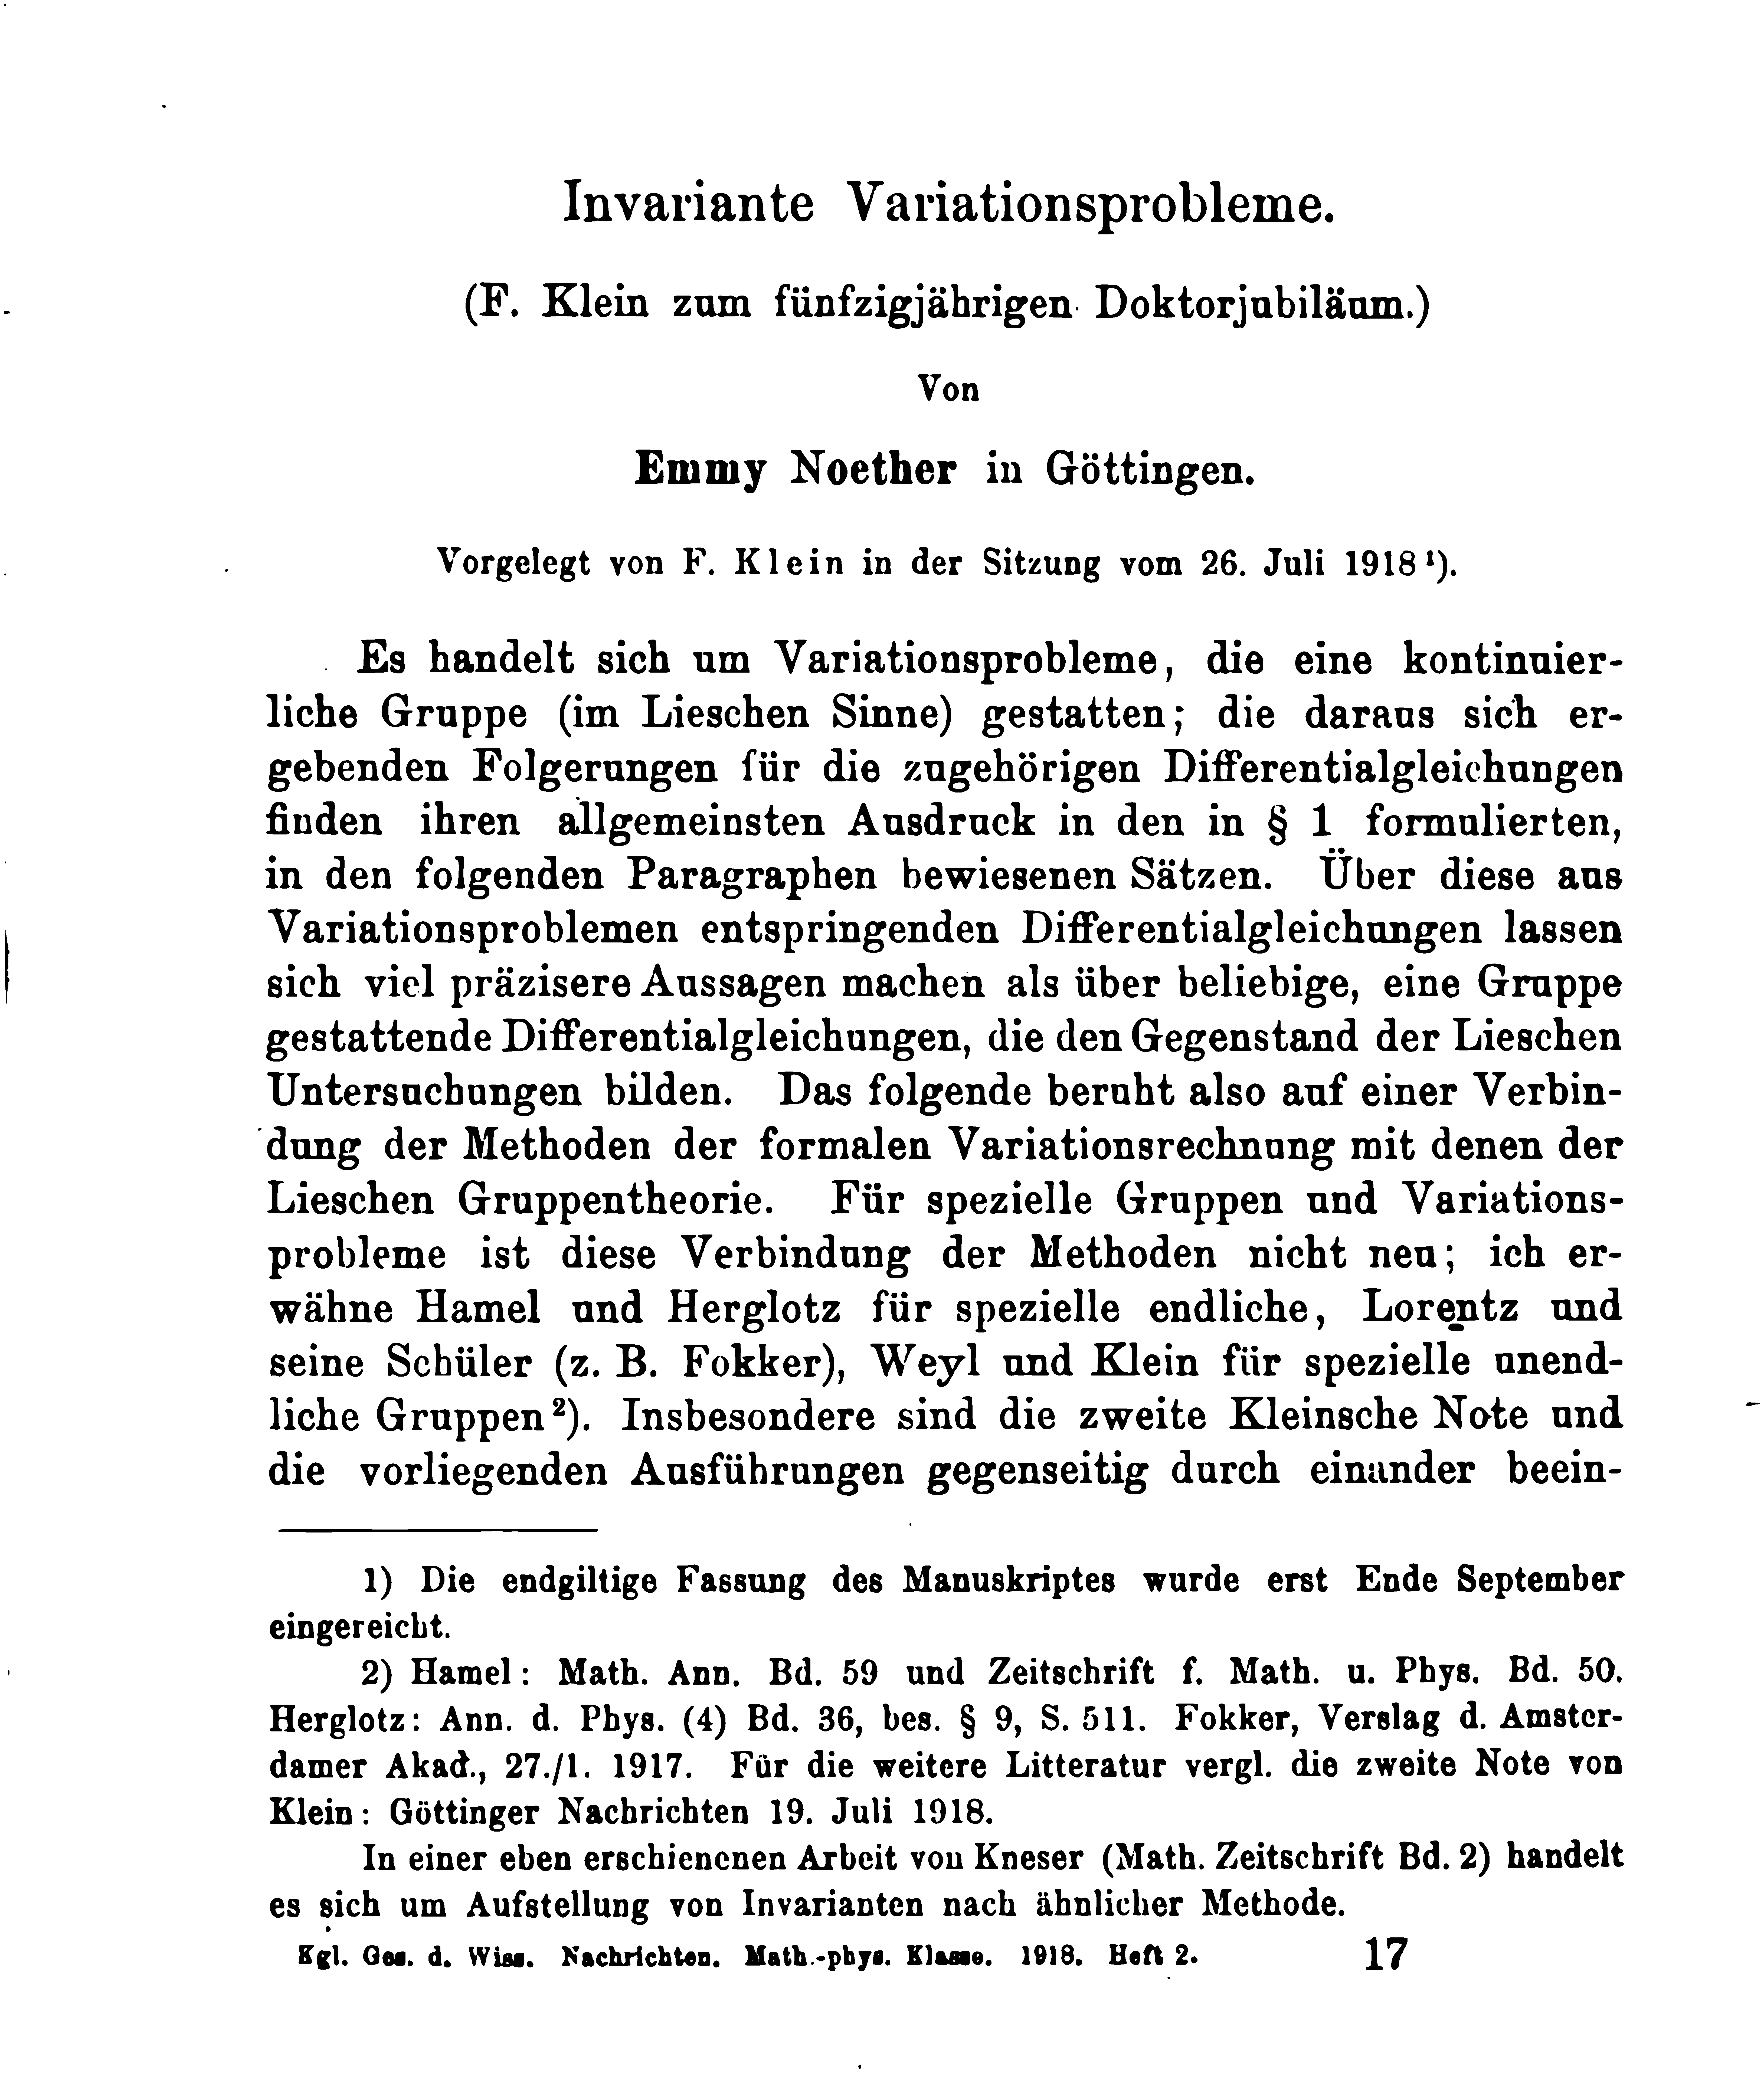
\includegraphics[scale=0.06]{Articulo_de_Noether.eps}}
%	\caption{\textit{Artículo de Noether publicado en 1918 ``Invariante Variationsprobleme"} }
%	\label{figura2}
%\end{figure}
%%%%%%%%%%%%%%%%%%%%%%%%%%%%%%%%%
\section{Teorema de Noether}
\subsection{La Acción}
 Se representa la energía mediante la siguiente ecuación:
 
  \begin{equation}
      E=K(\dot{q})+V(q)
  \end{equation}
  
 donde \(K\) es energía cinética y  \(V\)  es la energía portencial. La energía cinética depende de la velocidad \((\dot{q})\), mientras que la energía potencial puede depender de la posición \((q)\). \\
 
 Se definie el Lagrangiano \((L)\) como:
 \begin{equation}
     L(q,\dot{q})=K(\dot{q})-V(q) 
 \end{equation}

En la dinámica lagrangiana, la conexión general entre las propiedades de simetría (invariancia) y las cantidades conservadas se establece mediante un importante teorema debido a Emmy Noether. \cite{Nivaldo}

 
Se presenta colectivamente el sistema mediante \( q = (q_1, q_2, \ldots, q_i)\) para las coordenadas generalizadas y  
 \( \dot{q} = (\dot{q}_1, \dot{q}_2, \ldots, \dot{q}_i) \) para las velocidades correspondientes. Donde \(q_i\) representa la i-ésima coordenada generalizada y \( \dot{q}_i\)  la velocidad asociada a esa coordenada. \\
 
 Con ello se puede hacer la representación del funcional \([S]\), como ``La acción"\cite{Nilo}
 \begin{equation}
     [S]=\int_{t}^{t'}  L(q,\dot{q},t) dt
 \end{equation}
  Se definie como la integral del Lagrangiano con respecto al tiempo. Una función de las trayectorias $q(t)$, gracias al Lagrangiano $(L)$.
  
El movimeinto del sistmea , se obtiene con el principio de acción mínima o también llamado principio de acción estacionaria, del cual establece que el movimiento real del sistema es tal que la variación de la acción es cero en los puntos final $t_1$ y $t_2$.
Las ecuaciones de movimiento son las conocidas ecuaciones de Euler-Lagrange:
\begin{equation}
   \frac{d}{dt} \frac{\partial L}{\partial \dot{q}_i} - \frac{\partial L}{\partial q_i} = 0, \quad i = 1, 2, 3, \ldots, n  
\end{equation}

El principio de mínima acción, fundamentado en la teoría lagrangiana de la mecánica, establece que la trayectoria seguida por un sistema físico entre dos puntos en el espacio-tiempo es aquella para la cual la acción es mínima. La acción se obtiene a partir del Lagrangiano del sistema, una magnitud que depende de las coordenadas y velocidades del sistema. Un cambio de en la elección de coordenadas se denomina transformación pasiva.\\

Durante una Transformación pasiva, al cambiar las coordenadas utilizadas para describir el sistema, la forma de las ecuaciones de movimiento específicas en las nuevas coordenadas cambia con respecto a las anteriores, pero el sistema en sí permanece inalterado. Es un ajuste en la perspectiva descriptiva, sin implicar cambios físicos reales en el sistema. En contraste, existen transformaciones muy especiales que también pueden considerarse en sentido activo, es decir, que representan cambios reales en el sistema, modificando sus propiedades o estados. Estas transformaciones tienen un impacto tangible en el sistema y pueden ser llevadas a cabo físicamente. La Invariancia de la Acción hasta una constante aditiva durante ciertas transformaciones es crucial. Estas transformaciones están vinculadas a cantidades que se conservan en el sistema.

  






 \subsection{Transformaciones de simetría Noetheriana}
Se considera un camino en la coordenada dado $q_i=q(t), \hspace{0.5cm} i=1,2, \ldots, n $ y se transfoma según
\begin{equation}
    q'_i= q_i+ \epsilon K_i(q,\dot{q},t) 
    \label{5}
\end{equation}

\begin{equation}
     t'=t+\epsilon\theta(q,\dot{q}, t)
\label{6}
\end{equation}


donde $\epsilon$ es una constante de parámetro infinitesimal.
Se deduce que es una transfomación activa, en la trayectoria $\gamma(q(t),t)$, esta mapeado en $\gamma'(q'(t'),t')$ En el caso de sistemas unidimensionales, se ilustra en la Fig[1].


%%%%%%%%%%%%%%%%%%%%%%%%%%%%%%%%%%%%%%%%%%%%%%%%%%%%%%%%%%%%%%%%%%%
% colocar imagen
%\begin{figure}
%	\centerline{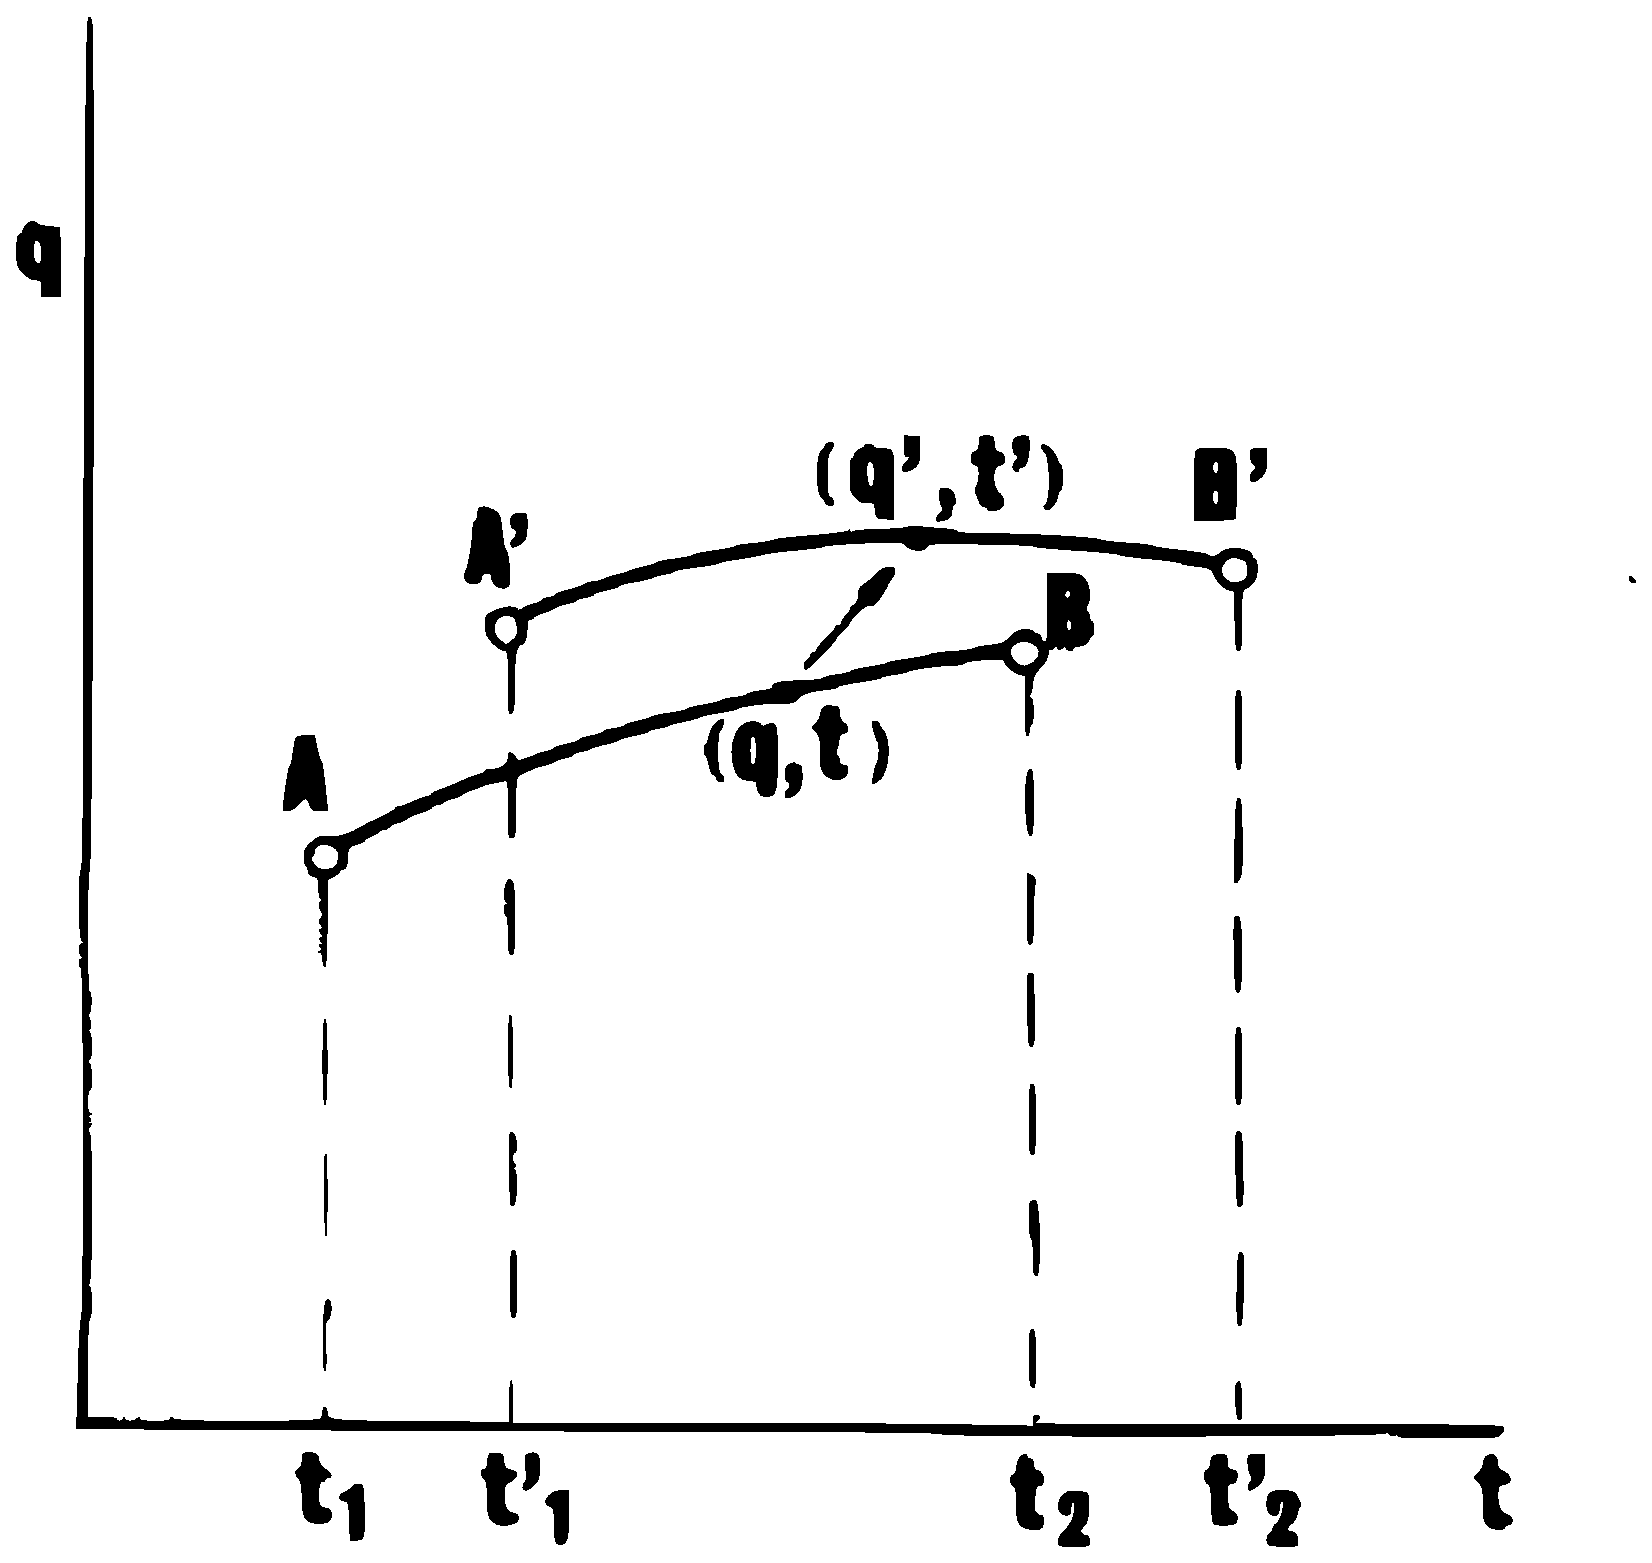
\includegraphics[scale=0.2]{grafica_3.eps}}
%	\caption{\textit{Efecto de una transformación de espacio y tiempo en la trayectoria de un sistema} }
%	\label{figura1}
%\end{figure}
        \begin{figure}[h]
         \centering{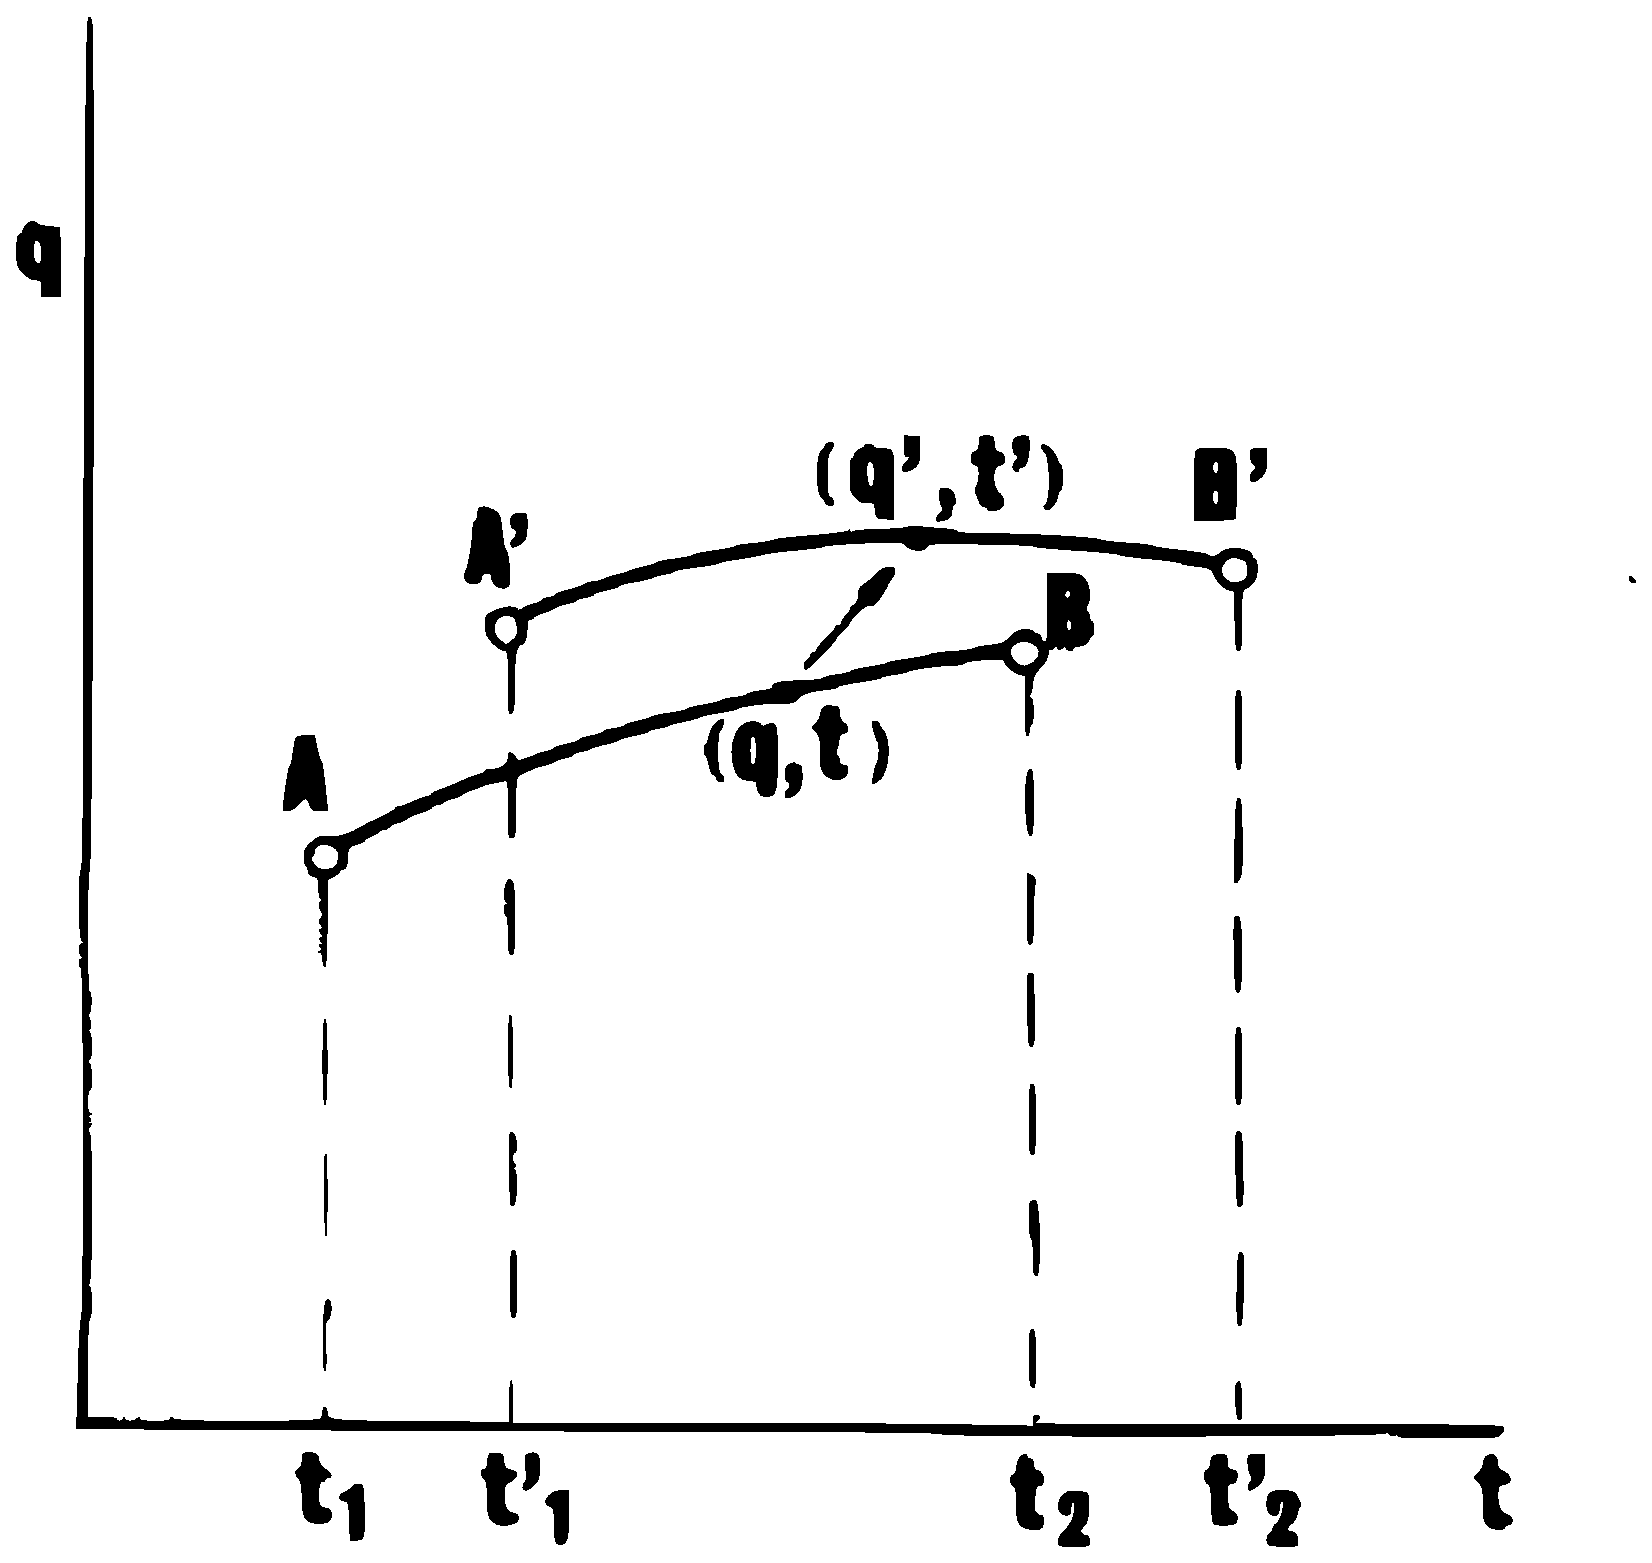
\includegraphics[scale=0.2]{grafica_3.eps}}
              \caption{\textit{Efecto de una transformación de espacio y tiempo en el camino de un sistema unidimensional.
              }}
          \label{figura2}
        \end{figure}

En donde se puede apreciar que los camino de $\gamma$ está en dos puntos $A$ y $B$ correspondiente a los puntos  $t_1$ y $t_2$, respectivamente. 
Entonces los puntos de la transformación entre $A'$ y $B'$ correspondiendo a los tiempos\cite{Nilo}

\begin{equation}
     t'_1=t+\epsilon\theta(q^a,\dot{q}^at_1)
\label{7}
\end{equation}

\begin{equation}
    t'_2=t+\epsilon\theta(q^b,\dot{q}^b,t_2)
\label{8}
\end{equation}

Condición suficiente para que las transformaciones en las ec.~(\ref{7}) y (\ref{8}) constituyan una transformación de simetría de la acción. Esto implica que la acción debe mantenerse constante, hasta el término de primer orden en $\epsilon{}$, a lo largo de las trayectorias $\gamma$ entre los puntos A y B, y $\gamma'$ entre los puntos $A'$ y $B'$. Es decir

\begin{equation}
    \int_{t'_1,\gamma}^{t'_2} L(q,\dot{q},t)dt =  \int_{t'_1,\gamma}^{t'_2} L(q',\dot{q}',t')dt' + O(\epsilon^2)
    \label{9}
\end{equation}


donde


\begin{equation}
    \dot{q}_i = \frac{dq_i}{dt} , \hspace{1cm} \dot{q}'_i=\frac{dq'_i}{dt'}
\end{equation}


En la ec.~$(\ref{9})$  establece que tanto un camino específico $\gamma$ como otro camino $\gamma'$ son trayectorias reales del sistema, ya que las acciones a lo largo de ambas trayectorias son iguales, alcanzando el mismo valor mínimo. Esto implica que ambos caminos comparten propiedades fundamentales y representan soluciones válidas para el sistema. Para hacer el análisis más flexible, la constante aditiva en la acción no afecta la condición mínima. 

Por lo tanto, podemos introducir una condición menos restrictiva en la cual solo consideramos términos de primer orden en una pequeña perturbación, representada por la energía $\epsilon$. Esta nueva condición se refiere a la consistencia de las trayectorias $\gamma$ y $\gamma'$ en términos de sus acciones, asegurando que, para términos de primer orden en $\epsilon$

\begin{equation}
    \int_{t'_1,\gamma}^{t'_2} L(q,\dot{q},t)dt =  \int_{t'_1,\gamma}^{t'_2} L(q',\dot{q}',t')dt' + \epsilon A + O(\epsilon^2)
\label{11}
\end{equation}

donde $A$ se representa 

\begin{equation}
A = f[q'(t'_2), t'_2] - f[q'(t'_1), t'_1] = \int_{t'_1}^{t'_2} \left(\frac{df(q', t')}{dt'} \right)\,dt'
\label{12}
\end{equation}

La función \(f\) no puede depender de \(q'\) ni de derivadas superiores porque \(A\) (la acción) debe permanecer constante bajo una variación de la trayectoria con \(q'(t'_1)\) y \(q'(t'_2)\) fijos. Esto significa que si cambiamos la trayectoria del sistema de alguna manera, manteniendo fijas las velocidades generalizadas en los puntos \(t'_1\) y \(t'_2\), la acción del sistema no debe cambiar.

La nueva trayectoria diferiría de la anterior en las velocidades generalizadas \(\dot{q}'\) en \(t'_2\). En otras palabras, si cambiamos la trayectoria del sistema, las velocidades generalizadas en el punto \(t'_2\) serían diferentes para la trayectoria original y la trayectoria modificada. Al sustituir \( A \), dado por la ec.~(\ref{12}) en la ec.~(\ref{11}), se obtiene

\begin{equation}
    \int_{t'_1,\gamma}^{t'_2} L(q,\dot{q},t)dt =  \int_{t'_1,\gamma}^{t'_2} L\left(q',\dot{q}',t'+\epsilon \frac{df(q',\dot{q}',t')}{dt'}\right)dt' + O(\epsilon^2)
\label{13}
\end{equation}

Cualquier transformación dada en las ec.~\((\ref{8})\) y \((\ref{7})\) tal que la ec.~\((\ref{13})\) sea válida para cualquier intervalo de tiempo \((t_1, t_2)\), cualquier camino \(\gamma\) y cualquier función \(f\) se denomina asimetría de transformaciones de Noether del sistema físico.



\subsection{Leyes de conservación de Noether}

La respresentación de la transformación Noetheriana esta representado por las ec.~(\( \ref{5} \)) y (\(\ref{6}\)), la cantidad 
\begin{equation}
    E=\sum_i p_i K_i - E\theta+f
\end{equation}


donde

\begin{equation}
    p_i=\frac{\partial L}{\partial \dot{q}_i}
\end{equation}


y 



\begin{equation}
    E= \sum_i p_i \dot{q}_i - L
\end{equation}

es conservado, es decir, permanece constante a lo largo de trayectorias reales del sistema. Para demostrar este teorema, se da el cambio en la variable de tiempo en el lado derecho de la ec.~(\(\ref{13}\)), en lugar de \(t'\), se utiliza \(t\), y consecuentemente, se ajustan los límites de la integral de \(t'_1\) y \(t'_2\) a \(t_1\) y \(t_2\), respectivamente. Del cual resulta

\begin{equation}
    \int_{t_1}^{t_2} L(q, \dot{q},t) dt = \int_{t_1}^{t_2} \left( L(q',\dot{q}',t') +\epsilon \frac{df(q',t')}{dt'}\right) \left(\frac{dt'}{dt} \right) dt
    \label{17}
\end{equation}

Este cambio facilita la comparación de ambos lados de la ec.~(\(\ref{13}\)) bajo esta nueva elección de variables. 
Lo que muestra que el valor considerado sigue siendo constante a los largo de las trayecotrias reales. 


Ahora, se transforma las variables de la ec.~(\(\ref{13}\)) de acuerdo con la ec.~(\(\ref{5}\)) y la ec.~(\(\ref{6}\)) 

\begin{equation}
    q'_i=\dot{q}_i+\epsilon(\dot{E}_i-\dot{\theta} \dot{q}_i), 
\end{equation}

\begin{equation}
    \frac{dt'}{dt}=1+\dot{\epsilon}
\end{equation}

se obtiene, hasta terminos de primer orden en \(\epsilon \)

\begin{equation}
     \int_{t_1}^{t_2} L(q, \dot{q},t) dt = \int_{t_1}^{t_2} \left[L(q,\dot{q},t) +\epsilon \left( \sum_i K_i \frac{\partial L}{\partial q_i} + \sum_i (\dot{K}_i - \dot{\theta} \dot{q}_i) \frac{\partial L}{\partial \dot{q}_i} +\theta\frac{\partial L}{\partial t} +\dot{\theta} L +\dot{f} \right) \right] dt
\label{20}
\end{equation}

Ambas ecuaciones de la ec.~$(\ref{20})$ se realizan  lo largo de trayectorias reales que satisfacen las euaciones de movimiento del sistema. De modo que, si \(p_i\) es movimiento canónico conjugado a \(q_i\), 

\begin{equation}
    p_i=\frac{\partial L}{\partial \dot{q}_i}
    \label{21}
\end{equation}

su derivada total respecto al tiempo está dada por

\begin{equation}
    \dot{q}_i = \frac{d}{dt} \frac{\partial L}{\partial \dot{q}_i} = \frac{\partial L}{\partial q_i}
    \label{22}
\end{equation}

Al sustituir la ec.~(\ref{21}) y la ec.~(\ref{22}) en la ec.~(\ref{20}), expresando \( \frac{\partial L}{\partial t} \) en términos de \( \frac{dL}{dt} \), \( \frac{\partial L}{\partial q} \) y usando la arbitrariedad de \(\epsilon\). La ec.~\(\ref{20}\) queda

\begin{equation}
    \int_{t_1}^{t_2} \left( \sum_i (\dot{p}_i K_i +p_i\dot{K}_i -p_i\dot{q}_i \dot{\theta}) -\dot{E}\theta +\dot{\theta} L +\dot{f} \right) dt = 0
    \label{23}
\end{equation}

Ahora, dado que \(t_1\) y \(t_2\) son completamente arbitrarios, en el término dentro de la integral en la ec.~(\(\ref{23}\)) se anula completamente 

\begin{equation}
      \sum_i (\dot{p}_i K_i +p_i\dot{K}_i -p_i\dot{q}_i \dot{\theta}) -\dot{E}\theta +\dot{\theta} L +\dot{f} = 0
\end{equation}

del cual se reescribe 

\begin{equation}
    \frac{d}{dt} \left( \sum_i p_i K_i - \theta E + f   \right) = 0
\end{equation}

el resultado se generaliza para transformaciones infenitesimales que dependen de parámetros independeintes \(\epsilon_{(\alpha)} (\alpha=1,2,\ldots,r)\) 

\begin{equation}
    q'_i=q_i+\sum_{(\alpha)} \epsilon_{(\alpha)} K^{(\alpha)} _i (q,t)
\end{equation}

\begin{equation}
     t'=t+\sum_{(\alpha)} \theta_{(\alpha)} K^{(\alpha)} _i (q,t)
\end{equation}

la transformación, al inetractuar sobre cualquier trayectoria real en el sistema, es tal igual que 

\begin{equation}
    \int_{t'_1}^{t'_2} L(q,\dot{q},t)dt =  \int_{t'_1}^{t'_2} \left( L (q',\dot{q}',t')+\epsilon \frac{df(q',\dot{q}',t')}{dt'}\right)dt' + O(\epsilon^2)
\end{equation}

se cumple, que el sistema presenta r leyes de conservación.

\begin{equation}
    \frac{d}{dt}\left(\sum_i p_i K^{(\alpha)}_i -E\theta_{(\alpha)} +f_{(\alpha)}  \right)=0 \hspace{0.5cm} (\alpha=1,2, \ldots, r )
\end{equation}

donde 

\begin{equation}
    E=\sum_i p_i \dot{q}_i - L
\end{equation}

este es el contenido del teorema de Noether.

 Siempre que las transformaciones de simetría sean tales que el tiempo se transforme de manera idéntica o, en el máximo escenario, sufra una translación uniforme

 \begin{equation}
    t'=t+\epsilon
\end{equation}

la ec.~(\(\ref{17}\)), es equivalente a 

\begin{equation}
    L(q,\dot{q},t)=L(q',\dot{q}',t') + \epsilon \frac{df(q',t')}{dt'}
\end{equation}


Esto es la condición de simetría dada en la mayoría de los libros de texto, y expresa la invariancia (generalizada) del Lagrangiano.
\section{Ejemplo}
\subsubsection{Conservación del momento en sistemas de partículas masivas aisladas}

El momento total \(\textbf{p}\) de un sistema aislado de partículas masivas se define como la suma de los momentos individuales de cada partícula, teniendo en cuenta las dependencias temporales de dichos momentos \cite{Smilga} 

\begin{equation}
    \sum_{i=1}^{N} p_i(t)=\textbf{p}.
    \label{33}
\end{equation}

donde \(\textbf{p}\) es una constante del tiempo. En la mecánica Newtoniana, indica que los momentos de las particulas cambian con el tiempo, que es consecuencia de la ley de gravitación.
\\

La ec. \ref{33} es invariante bajo traslación, lo que significa que su forma no cambia si se cambia el sistema de referencia espacial. También es covariante bajo rotaciones y operaciones de impulso aplicadas a los momentos de las partículas individuales, por lo tanto su forma se mantiene constante bajo estas transformaciones. 
Es covariante bajo el escalado conforme de los momentos de las partículas individuales. Esto implica que la forma de la ecuación no cambia si se multiplican los momentos de las partículas por un factor constante. Esto implica que la ley de conservación del momento no está asociada a masas particulares de partículas.
Un momento de una partícula  que depende del tiempo, genera una fuerza igual a la derivada temporal de este impulso. Dado que el momento se conserva , las fuerzas de las particulas se equilibran. 

\begin{equation}
    \textbf{P}_1 (t)=\textbf{p} -\sum_{i=2}^{N} p_i(t)
\end{equation}

la trayectoria de la partícula 1 está completamente determinada por los momentos dependientes del tiempo de las partículas 2 a \(N\), junto con la posición y el momento de la partícula 1 en \(t=0\). La conservación del impulso total guía este comportamiento. La presencia de las partículas vecinas parece doblar la trayectoria de la partícula 1, sugiriendo la generación de un campo gravitacional virtual por las partículas 2 a \(N\). Aunque este campo es virtual, su estructura se puede medir observando las trayectorias de la partícula 1, y se plantea desarrollar una descripción teórica de este campo y sus implicaciones físicas, siguiendo el enfoque de Einstein en la relatividad general

\section{Discuciones}
Se comprendió que las transformaciones de simetría actuaban sobre trayectorias en lugar de puntos específicos en el espacio y el tiempo, exponiendo así la conexión intrínseca entre simetrías y leyes de conservación. En la sección de ``La Acción", se abordaron conceptos clave, como el Lagrangiano y el Principio de Acción Mínima, que establecieron la base para la aplicación del teorema de Noether. En ``Transformaciones de simetría Noetheriana", se resaltaron las transformaciones que mapeaban trayectorias en lugar de puntos discretos en el espacio y el tiempo, y se introdujo el concepto de invariancia de la acción hasta una constante aditiva durante transformaciones específicas. Esto proporcionó un marco conceptual sólido para la derivación de las leyes de conservación. En ``Leyes de conservación de Noether", se derivaron de manera general las cantidades conservadas que resultaban de las simetrías inherentes a un sistema físico. Finalmente, en el ejemplo específico de la ``Conservación del momento en sistemas de partículas masivas aisladas", se mostró una aplicación concreta de las leyes de conservación derivadas del teorema de Noether, revelando cómo la conservación del momento guiaba las trayectorias individuales de las partículas y sugería la presencia de un campo gravitacional virtual.
































%%%%%%%%%%%%%%%%%%%%%
%\section{Apliaciones}



%%%%%%%%%%%%%%%%%%%%%%%%%%%%
%\section{Resultados y Discusión}



%%%%%%%%%%%%%%%%%%%%%%%%%%
%\section{Conclusiones}



%%%%%%%%%%%%%%%%%%%%%%%
%\section{Agradecimientos}









%%%%%%%%%%%%%%%%%%%%%%%%
\begin{thebibliography}{99}
%\bibitem{1} N. Apellido. Titulo del artículo. Rev. Inv. Fis., \textbf{21}(1), 18-26 (2018).

\bibitem{Volker} R. Volker. Noether. arXiv preprint math/0206043, (2002).    doi:\url{https://doi.org/10.48550/arXiv.math/0206043}


\bibitem{Valenzuela} B. Valenzuela. Emmy Noether por Belén Valenzuela Requena. Revista española de física, \textbf{32}(1), 56-63 (2018).

\bibitem{Goldstein} H Goldstein, Classical Mechanics. \textbf{2}. 588-596. (1980).

\bibitem{Hill} Hill E. L.Hamilton's Principle and the Conservation Theorems of Mathematical Physics. Rev. Mod. Phys. \textbf{23} 253-260 (1951). doi: \url{https://doi.org/10.1103/RevModPhys.23.253}

\bibitem{Freire} N. Freire. Emmy Noether y su inigualable legado matemático. National Geographic. (2023)

\bibitem{Nilo} A. Nilo B.. Noether’s theorem in discrete classical mechanics. Am. J. Phys. \textbf{56} 174–177 (1988). 
doi:\url{https://doi.org/10.1119/1.15700}

\bibitem{Nivaldo} A. Nivaldo. Analytical Mechanics. Cambridge University Press. \textbf{2} (2018)

\bibitem{Smilga} W. Smilga. Noether's Theorem, Conservation of Momentum, and Gravitation in Isolated Multiparticle Systems. ResearchGate (2022)
doi: \url{http://doi.org/10.13140/RG.2.2.10686.97603}


\end{thebibliography}

\end{document}
